\documentclass[9pt]{beamer}
\mode<presentation>
\usepackage[T1]{fontenc}
\usepackage{color}
\usepackage{graphicx}
\usepackage{natbib}
\usepackage{tikz}
\usetikzlibrary{shapes.geometric}
\usepackage{xmpmulti}
\usepackage{animate}
\usepackage{tcolorbox}
\usepackage{amsmath}
\usepackage{gensymb}
\usepackage{csquotes}
\usepackage{bibentry}
\nobibliography*

\usetheme{Singapore}

\setbeamercolor{block title}{bg=structure!20}
\setbeamercolor{block body}{bg=structure!10}
\setbeamertemplate{blocks}[rounded][shadow]
\setbeamertemplate{caption}{\raggedright\insertcaption\par}
%\usecolortheme{seahorse}

\usefonttheme{professionalfonts}



\title[Climate Policy Instruments]{What is the evidence on climate mitigation policies, and to what extent can it be identified and classified using Machine Learning?}
\author{Max Callaghan}
\institute[MCC]{
	\includegraphics[height=1cm,width=2cm]{images/MCC_Logo_RZ_rgb.jpg} \hspace{5em} 
}
\date{}
\newif\ifframeinlbf
\frameinlbftrue
\makeatletter
\newcommand\listofframes{\@starttoc{lbf}}
\makeatother

\addtobeamertemplate{frametitle}{}{%
	\ifframeinlbf
	\addcontentsline{lbf}{section}{\protect\makebox[2em][l]{%
			\protect\usebeamercolor[fg]{structure}\insertframenumber\hfill}%
		\insertframetitle\par}%
	\else\fi
}

\newtheorem*{remark}{}

\bibliographystyle{apalike}

\begin{document}
	
\begin{frame}
	\titlepage
\end{frame}


%%%%%%%%%%%%%%%%%%%%%%%%%%%%%%%%%%%%%%%%%%%%%%%%%%
%% Introduction
\section{Introduction}

%\begin{frame}
%\tableofcontents[currentsection]
%\end{frame}

\begin{frame}{Context}

\begin{columns}
	\begin{column}{0.618\linewidth}
		\only<1>{\begin{figure}
			\includegraphics[width=\linewidth]{images/pathways}
			\caption{AR6 WGIII Fig 3.6}
		\end{figure}}
		\only<2->{\begin{figure}
		\includegraphics[width=\linewidth]{images/Figure_1.pdf}
		\caption{\cite{callaghan_topography_2020}}
\end{figure}}
	\end{column}
	\begin{column}{0.382\linewidth}
		\begin{itemize}
			\item<1-> Meeting Paris goals requires an extremely rapid reversal of >100 years of rising emissions, going far beyond existing policies
			\item<2-> The amount of climate policies, and the size of the scientific literature on policies is growing fast
			
		\end{itemize}
	\only<3->{\begin{remark}
		What instruments are studied where? How does this match with enacted instruments and emissions data?
	\end{remark}}
	\end{column}
\end{columns}

\end{frame}

\begin{frame}{Plan}

What is the evidence on climate mitigation policies, and to what extent can it be identified and classified using Machine Learning?

\medskip

A machine-learning-assisted systematic map

\begin{itemize}
	\item Develop a typology of climate policy instruments
	\item Screen and code documents by hand
	\item Predict labels for all other documents
	\item Extract geolocations
	\item Produce a map of what types of instruments we study in what places
	\item Bring this information together with policy databases / emissions
\end{itemize}
\end{frame}


\section{Typology}
\begin{frame}{Typology}

\begin{figure}
	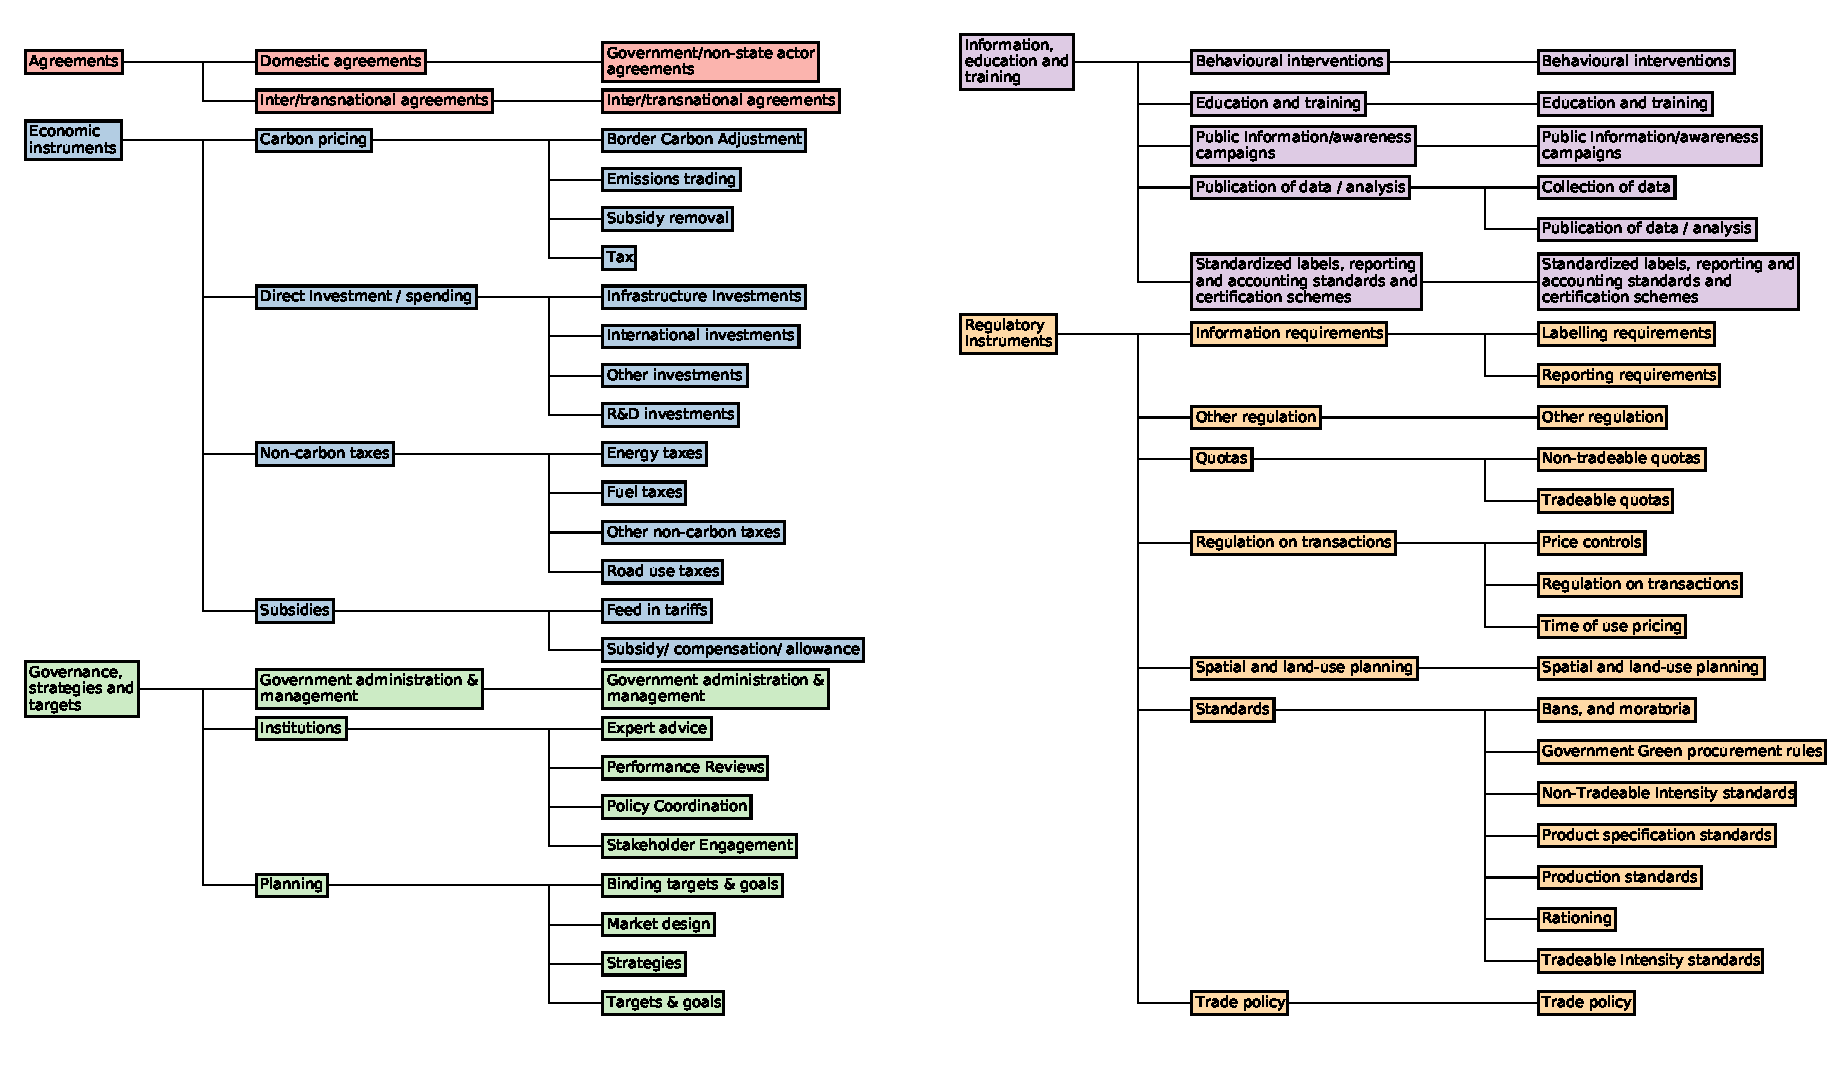
\includegraphics[width=\linewidth]{../figures/typology_wide.pdf}
\end{figure}
\end{frame}

\begin{frame}{Typology in context}
\begin{columns}
	\begin{column}{0.618\linewidth}
		\begin{figure}
			\only<1>{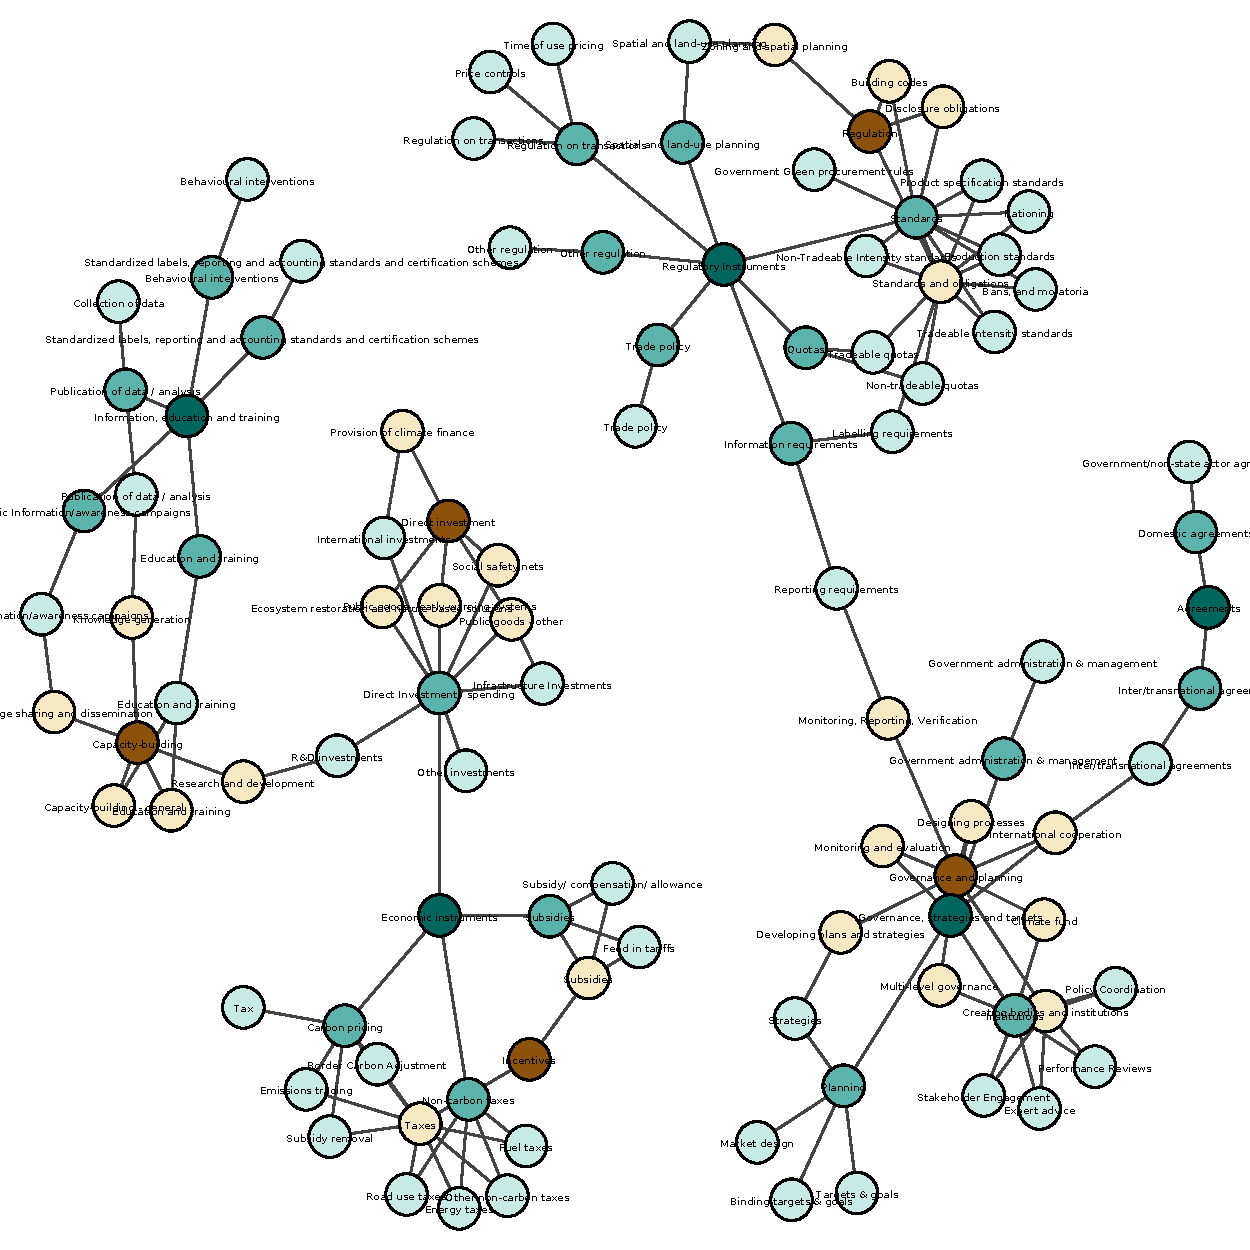
\includegraphics[width=\linewidth]{../figures/grantham_mcc.pdf}}
			\only<2>{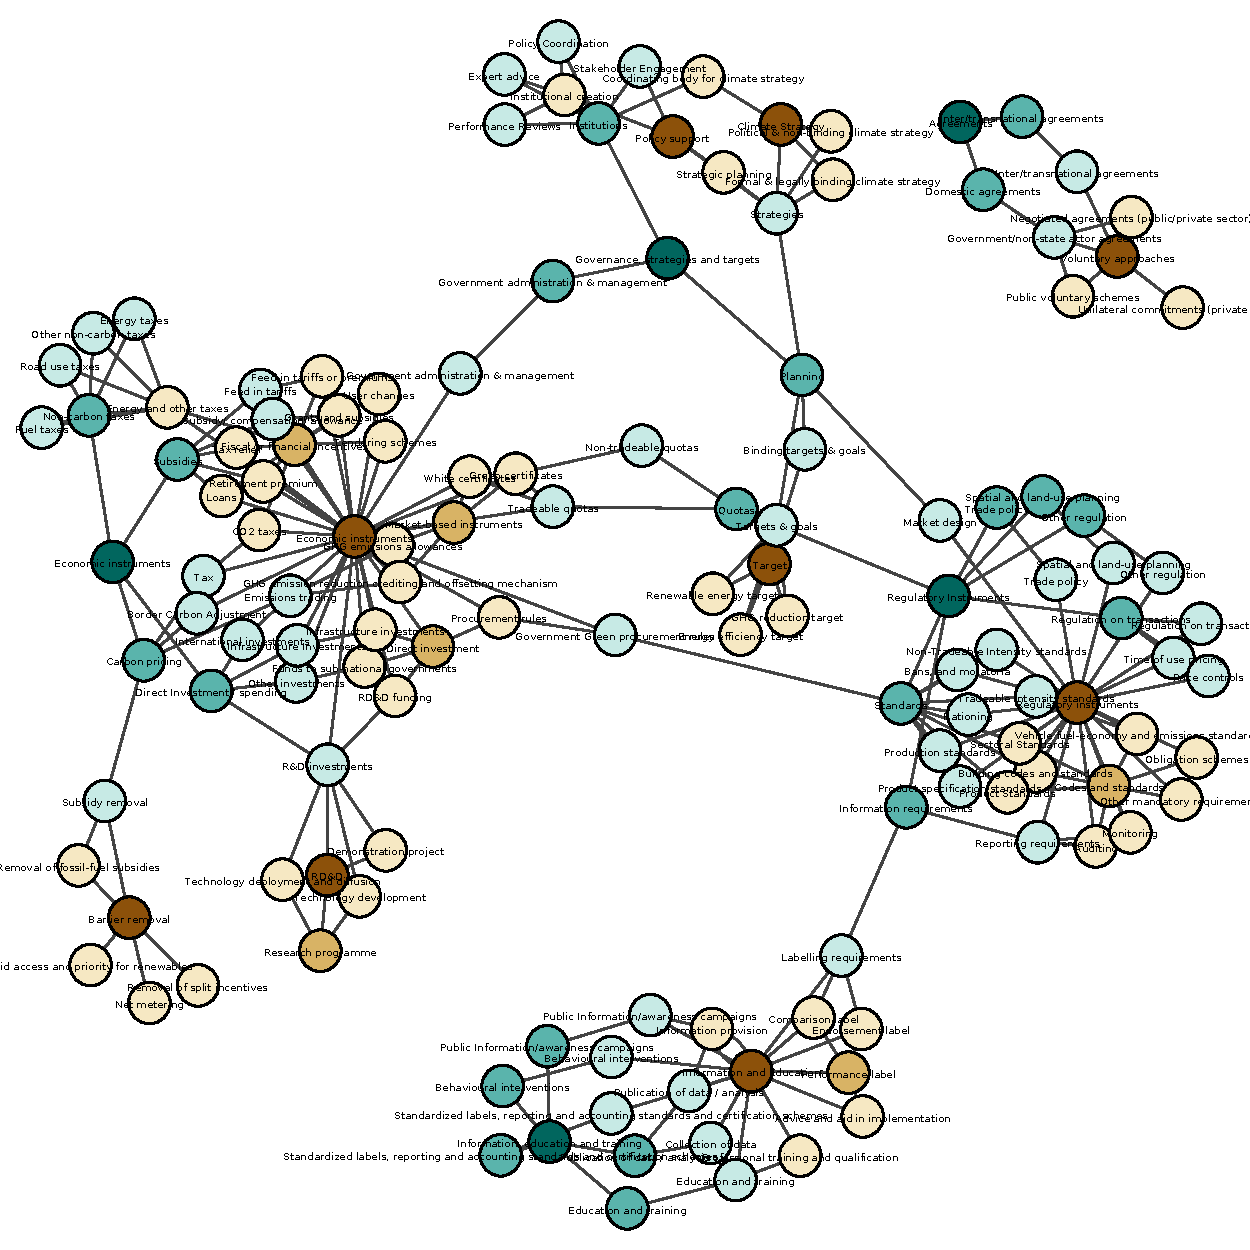
\includegraphics[width=\linewidth]{../figures/nci/g.pdf}}
		\end{figure}
	\end{column}
	\begin{column}{0.382\linewidth}
		\begin{itemize}
			\item<1-> Our typology is more detailed than \citep{grantham_research_institute_on_climate_change_and_the_environment_climate_2022}
			\item<2-> We provide slightly more detail than \citep{new_climate_institute_database_2020} with a [subjectively] clearer hierarchy
		\end{itemize}
	\end{column}
\end{columns}
\end{frame}

\section{Methods}
\begin{frame}{Screening}
\begin{columns}
	\begin{column}{0.382\linewidth}
		\begin{itemize}
			\item<1-> In addition to the policy type, we coded sector, scale, and study type (ex-post/ex-ate + qual/quantitative)
			\item<2-> We double coded around 2,500 documents
			\item<3-> Each document took on average <3 minutes to code, total work is 310 person hours (just initial coding)
		\end{itemize}
	\end{column}
	\begin{column}{0.618\linewidth}
		\begin{figure}
			\only<1>{\includegraphics[width=\linewidth]{images/screenshot.png}}
			\only<2>{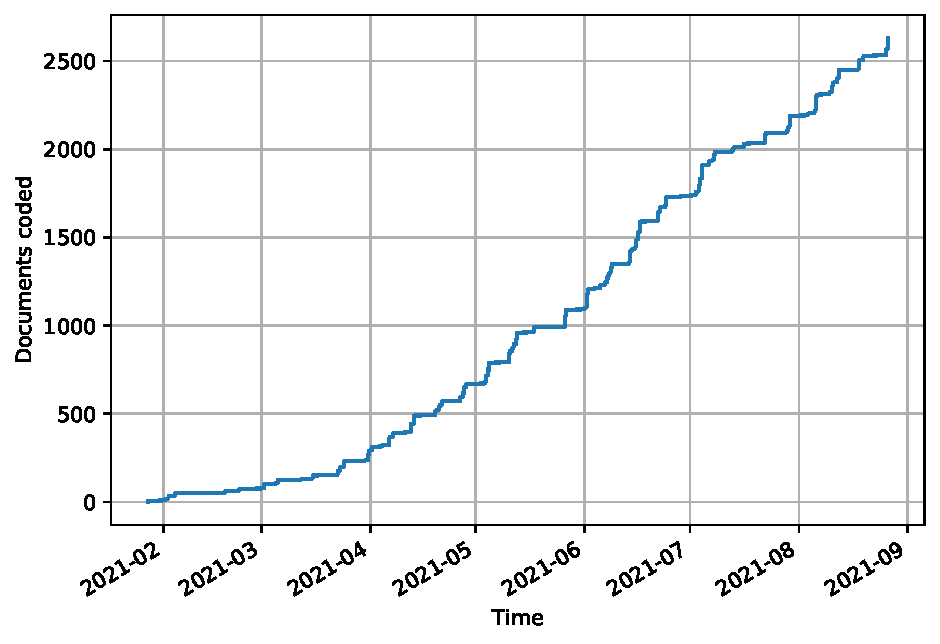
\includegraphics[width=\linewidth]{../figures/documents_screened_timeline.pdf}}
			\only<3>{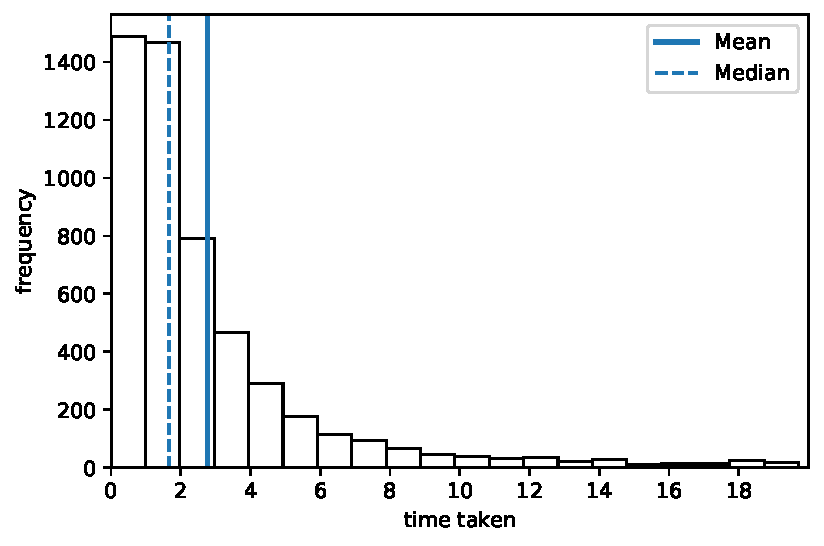
\includegraphics[width=\linewidth]{../figures/time_taken.pdf}}
		\end{figure}
	\end{column}

\end{columns}
\end{frame}

\begin{frame}{ClimateBert}

BERT (Bidirectional Representations from Transformers) is trained (by Google) on huge text corpora, and can be \textbf{``fine tuned''} on custom tasks. \cite{webersinke_climatebert_2021} perform additional pre-training on texts from the climate domain.

\begin{figure}
	\includegraphics[width=\linewidth]{images/bert-transfer-learning.png}
	\caption{Source: \url{https://jalammar.github.io/illustrated-bert/}}
\end{figure}



\end{frame}



\begin{frame}{Validation}
\begin{columns}
	\begin{column}{0.682\linewidth}
		\begin{figure}
			\includegraphics[width=\linewidth]{images/si_figure_2.pdf}
		\end{figure}
	\end{column}
	\begin{column}{0.318\linewidth}
		\begin{itemize}
			\item Nested cross-validation separates hyperparamter optimisation from evaluation
			\item Less subject to random selection of test set in a test-validation-train setting
			\item Allows use of more data in a data-scarce setting
		\end{itemize}
	\end{column}
\end{columns}
\end{frame}

\begin{frame}{Uncertain predictions}



\begin{columns}
	\begin{column}{0.382\linewidth}
		\begin{itemize}
			\item In a previous study we made multiple predictions with multiple subsets of the data, and calculated the mean $\pm$ standard deviation for each sample.
			\item This captures some uncertainty from sensitivity of model to training data, but uses no information about model performance
			\item How to express uncertainty about model performance? 
		\end{itemize}
	\end{column}
	\begin{column}{0.618\linewidth}
		\begin{figure}
			\includegraphics[width=\linewidth]{images/predictions_unseen.png}
		\end{figure}
	\end{column}

\end{columns}

\end{frame}

\section{Results}

\begin{frame}{Results}
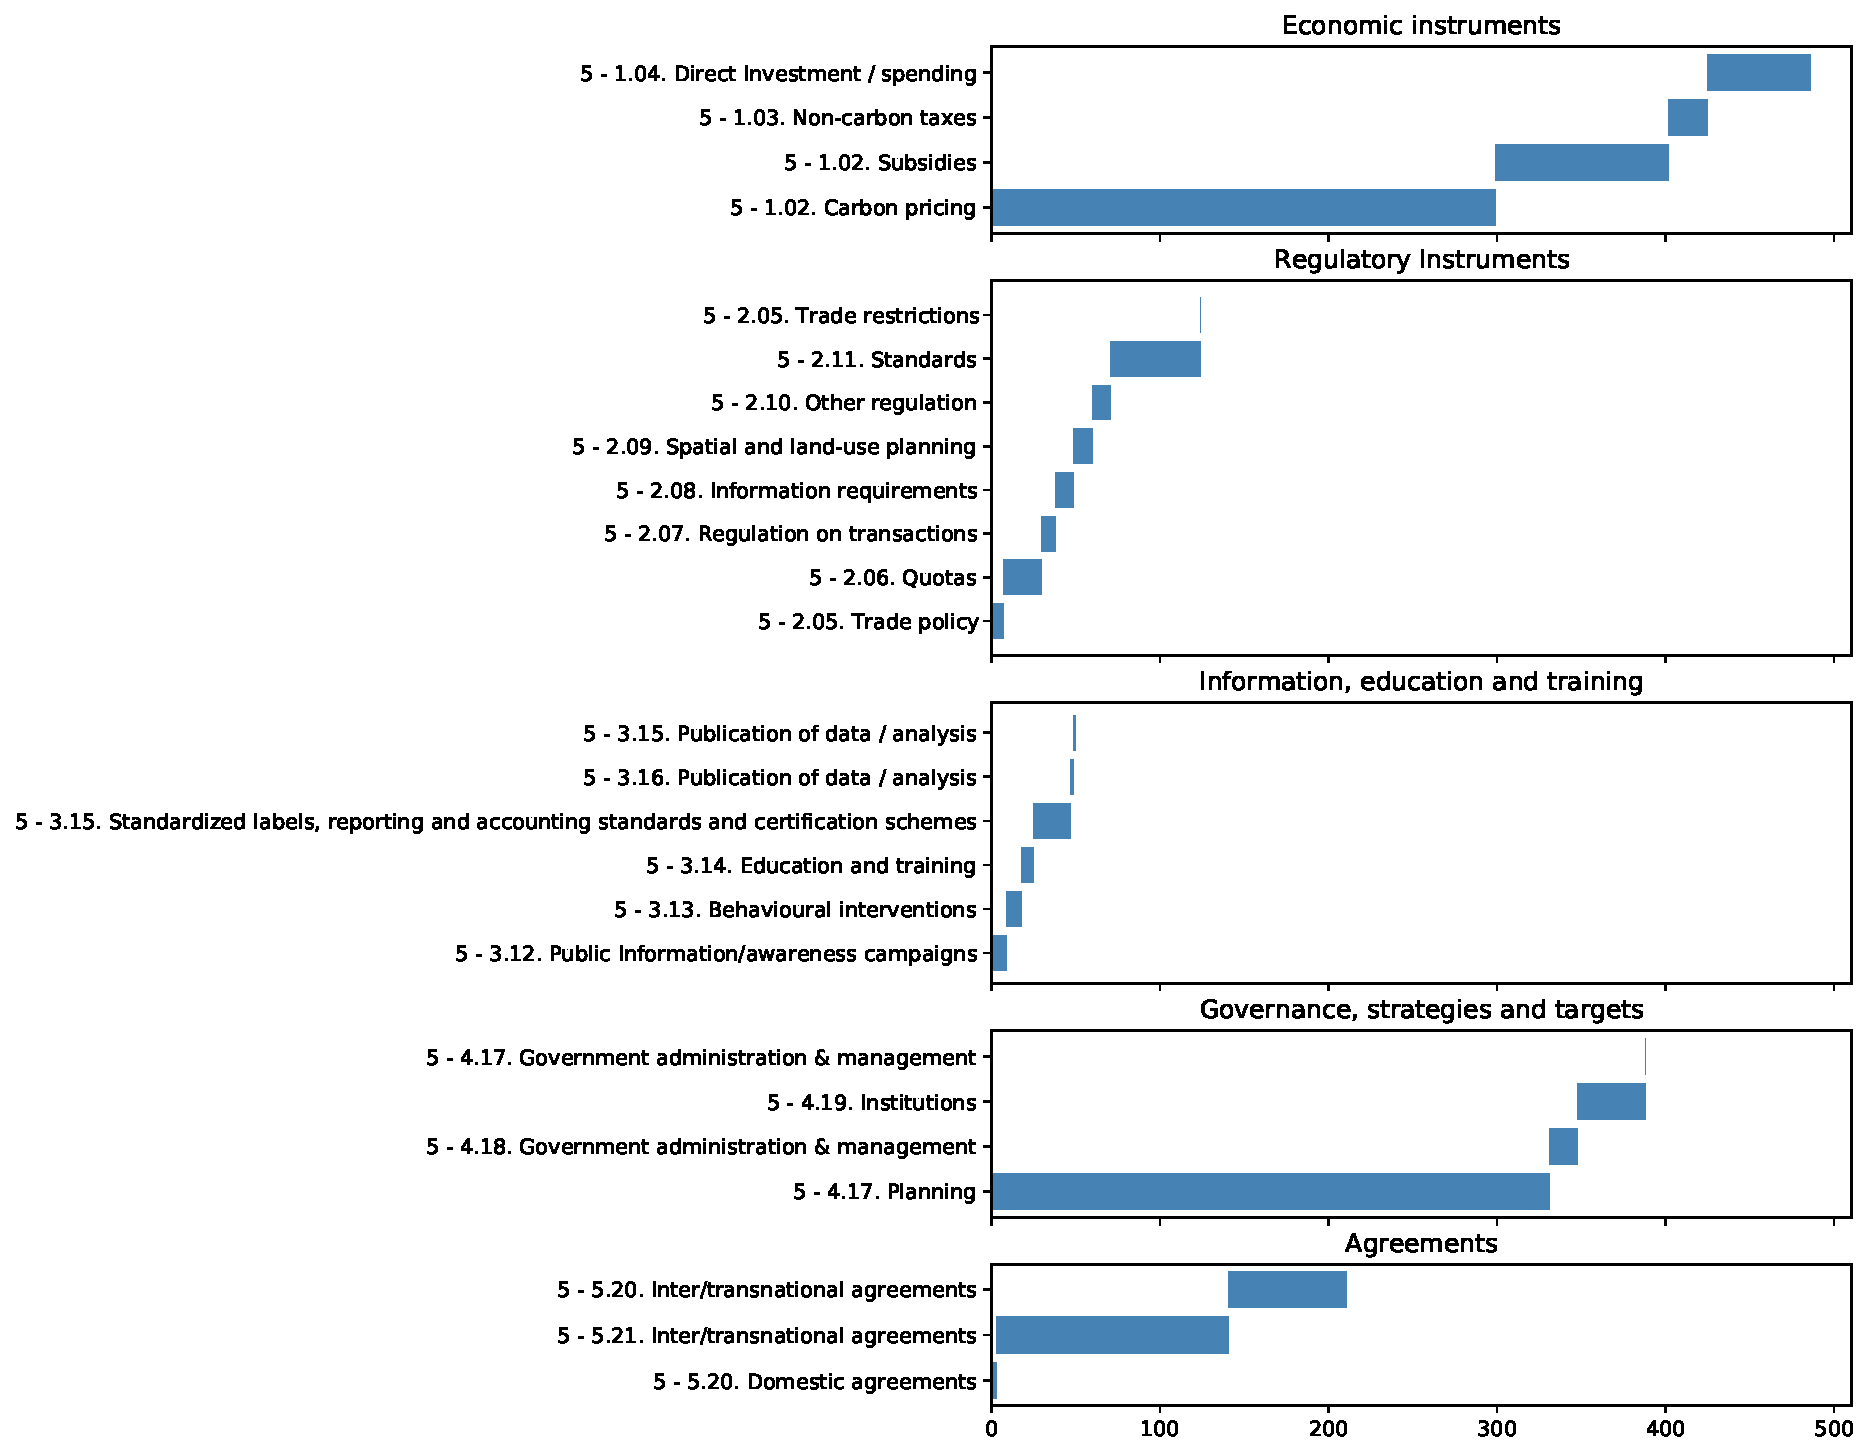
\includegraphics[width=\linewidth]{../figures/policy_counts.pdf}

\end{frame}

\begin{frame}{Human accuracy}

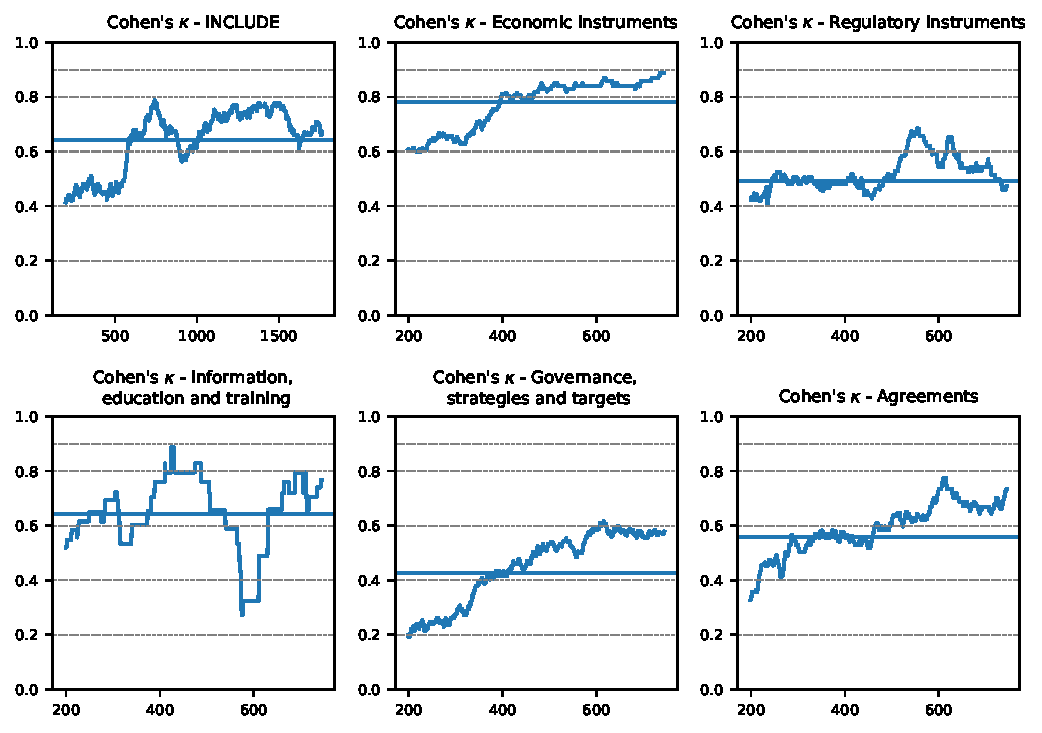
\includegraphics[width=\linewidth]{../figures/agreement_categories.pdf}

\end{frame}

\begin{frame}{CV results}

\begin{columns}
	\begin{column}{0.618\linewidth}
		\only<1>{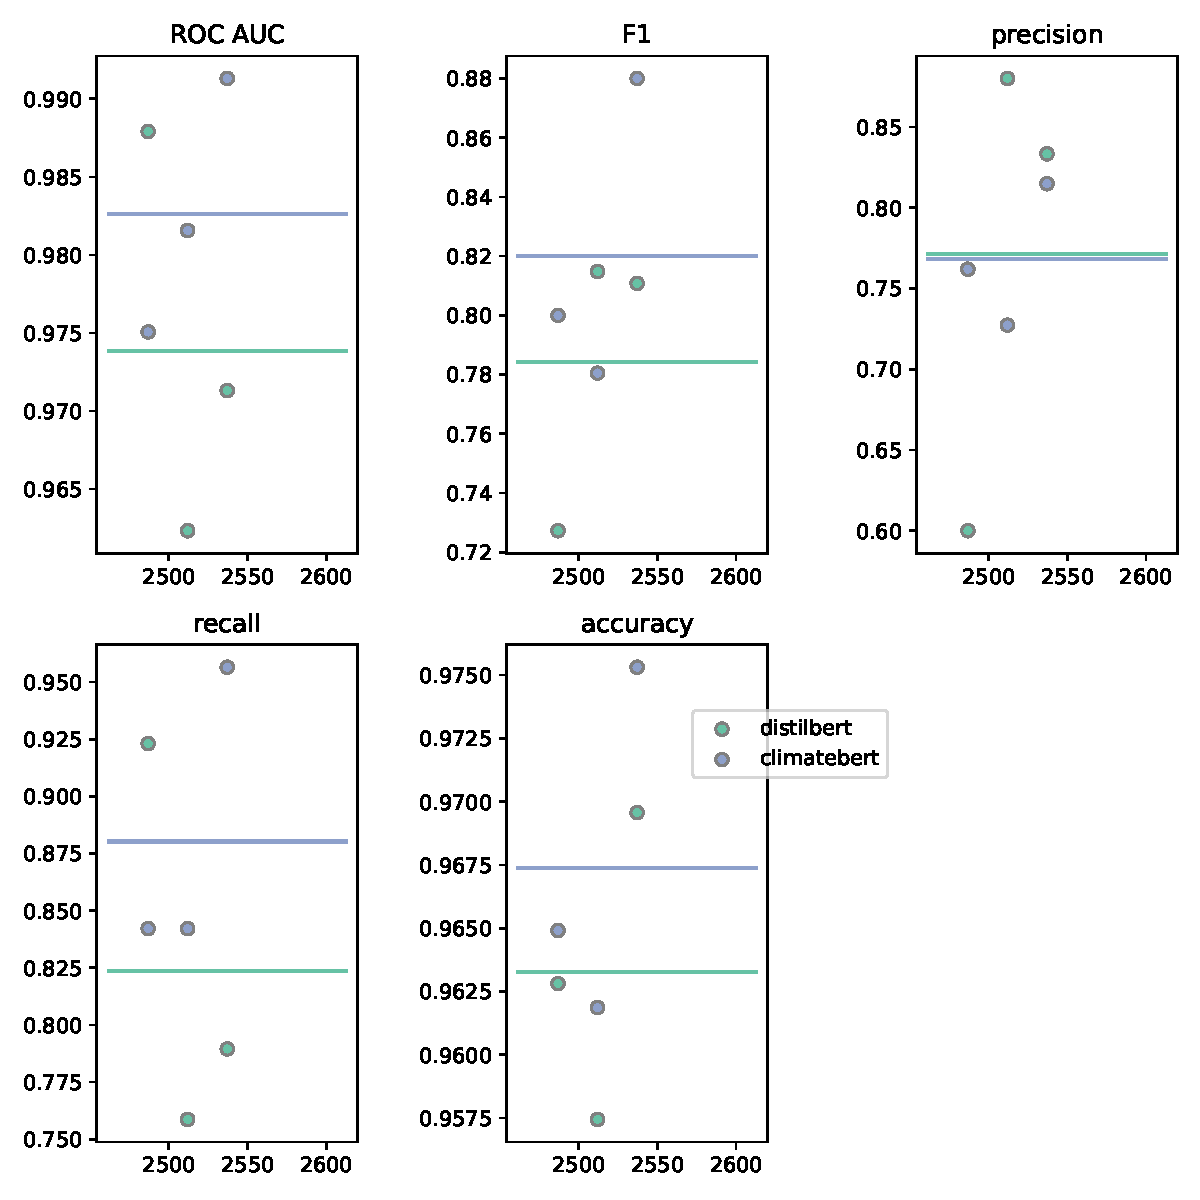
\includegraphics[width=\linewidth]{../figures/INCLUDE_metrics.pdf}}
		\only<2>{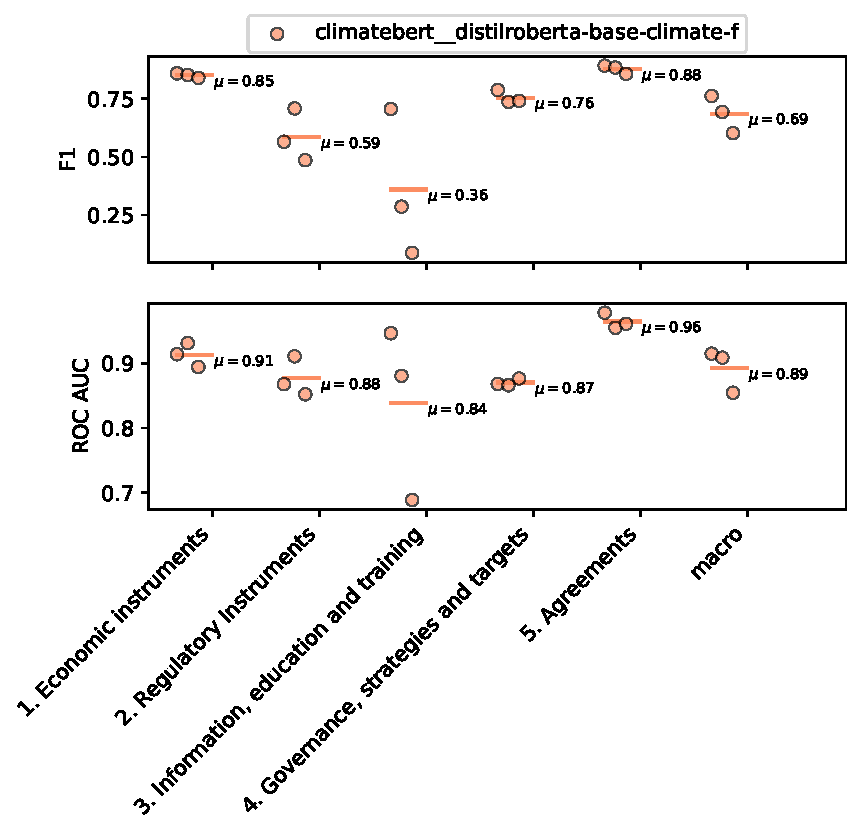
\includegraphics[width=\linewidth]{../figures/4_metrics.pdf}}
		\only<3>{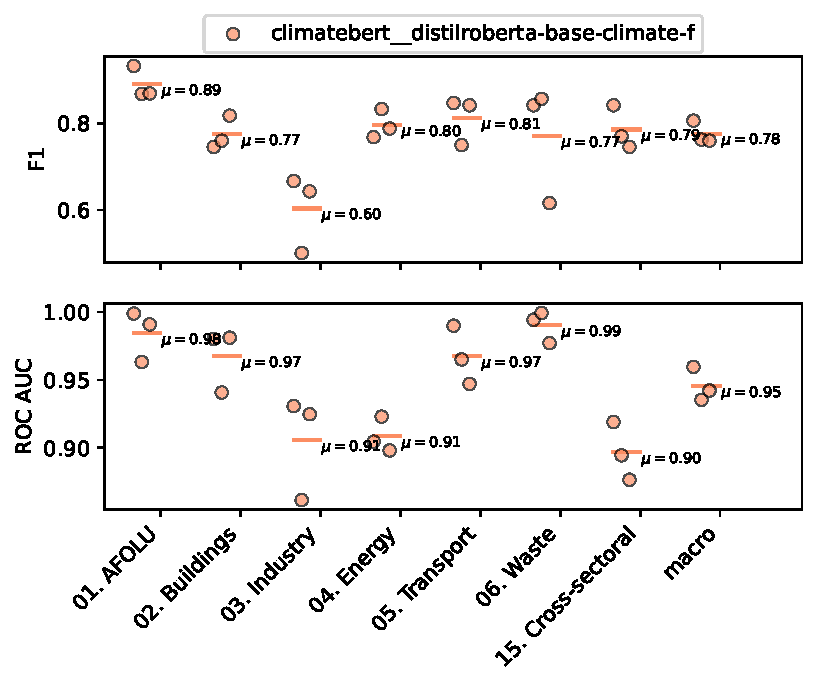
\includegraphics[width=\linewidth]{../figures/8_metrics.pdf}}
	\end{column}
	\begin{column}{0.382\linewidth}
		\begin{itemize}
			\item<1-> Inclusion is pretty well predicted%, with ROCAUC > F1 suggesting a poorly calibrated decision boundary
			\item<2-> We are poor at predicting classes with fewer samples
			\item<3-> Sectors are relatively well predicted
		\end{itemize}
	\end{column}
\end{columns}


\end{frame}

\begin{frame}{Geoparsing accuracy}

\begin{columns}
	\begin{column}{0.618\linewidth}
	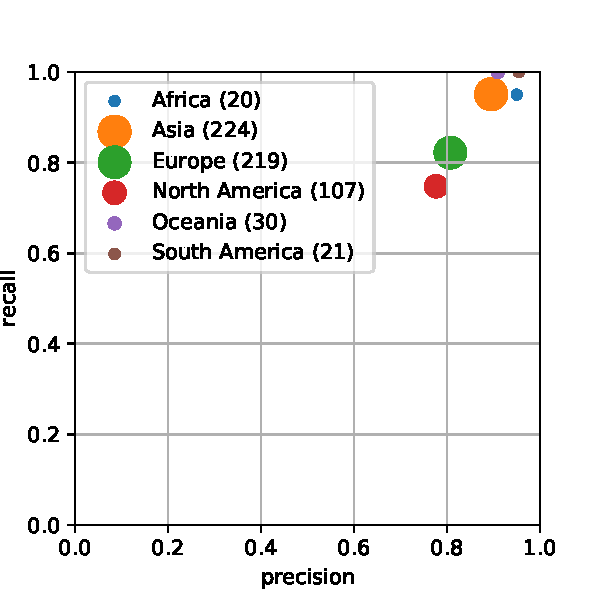
\includegraphics[width=\linewidth]{../figures/place_accuracy.pdf}
	\end{column}
	\begin{column}{0.382\linewidth}
		\begin{itemize}
			\item A combination of a geoparser for places, and a simple dictionary of country adjectives achieves good results
			\item That results are more accurate for Africa and Asia than Europe and North America is a pleasant surprise
		\end{itemize}
	\end{column}
\end{columns}

\end{frame}

\begin{frame}{Possible questions}

\begin{itemize}
	\item How does policy literature relate to policy databases?
	\item How does policy literature (+ policy databases) relate to emissions?
	\item Can learning across domains (policy + scientific docs) improve classifiers?
\end{itemize}

\end{frame}


%%%%%%%%%%%%%%%%%%%%%%%%%%%%%%%%%%%%%%
%%%%%%%%%%%%%%%%%%%%%%%%%%%%%%%%%%%%%%

%\begin{frame}{}
%
%\begin{columns}
%	\begin{column}{0.618\linewidth}
%	\end{column}
%	\begin{column}{0.382\linewidth}
%	\end{column}
%\end{columns}
%
%\end{frame}

%%%%%%%%%%%%
%% Bib
\begin{frame}{Bibliography and further resources}

\bibliography{climate-policy-instruments}
\end{frame}


\end{document}